To test the validity of the derived symmetries numerically, a curve fitting test based on the defining property of symmetries was conducted. A symmetry is defined by the fact that it maps one solution curve to another solution curve, and the test was implemented on the $t$-directional symmetries for the PLM as well as the IM-II. More specifically, the numerical validation was conducted in order to verify that the PLM given by

$$R(t)=At^{\gamma}$$

has a scaling-symmetry given by
\begin{equation}
\Gamma_{1,1}(\epsilon):(t,R)\mapsto \left(te^{\epsilon},R\right)
\label{eq:scaling}
\end{equation}
and that the IM-II given by

$$R(t)=\dfrac{A}{\exp\left(e^{-\alpha(t-\tau)}\right)-1}$$
has a symmetry given by
$$\Gamma_2(\epsilon):(t,R)\mapsto\left(\tau-\dfrac{\ln\left(\ln\left(\left|\alpha\epsilon-\exp\left(e^{-\alpha (t-\tau)}\right)\right|\right)\right)}{\alpha},R\right).$$
In this section, the principles of the validation will be presented in detail for the PLM but the same steps are analogous for the IM-II.

For the PLM, the parameter $\gamma$ is kept fixed as it determines the family of curves while the parameter $A$ is estimated as it specifies the specific curve. Now, the validation is started by obtaining a specific curve $R(t)=A_0t^{\gamma}$ for some fixed value $A_0$ and then a time series is generated from this curve by gathering $m\in\mathbb{N}_+$ realisations of this curve in a vector as follows

$$\mathbf{t}_0=\begin{pmatrix}t_1\\t_2\\\vdots\\t_m\end{pmatrix}\;\;\mathrm{and}\;\;\mathbf{R}_0=\begin{pmatrix}A_0t_1^{\gamma} \\A_0t_2^{\gamma}\\\vdots\\A_0t_m^{\gamma}\end{pmatrix}=\begin{pmatrix}R_1 \\R_2\\\vdots\\R_m\end{pmatrix}.$$
Next, the scaling symmetry $\Gamma_{1,1}(\epsilon)$ in \eqref{eq:scaling} is applied to the time series given by $\mathbf{t}_0$ and $\mathbf{R}_0$ which yields a new time series determined by the transformation parameter $\epsilon$. Denote this transformed time series by $\mathbf{\hat{t}}_0(\epsilon)$ and $\mathbf{\hat{R}}_0(\epsilon)$ respectively and this time series looks as follows
$$\mathbf{\hat{t}}_0(\epsilon)=\begin{pmatrix}\hat{t}_1(\epsilon)\\\hat{t}_2(\epsilon)\\\vdots\\\hat{t}_m(\epsilon)\end{pmatrix}=\begin{pmatrix}t_1e^{\epsilon}\\t_2e^{\epsilon}\\\vdots\\t_me^{\epsilon}\end{pmatrix}\;\;\mathrm{and}\;\;\mathbf{\hat{R}}_0(\epsilon)=\begin{pmatrix}\hat{R}_1(\epsilon) \\\hat{R}_2(\epsilon)\\\vdots\\\hat{R}_m(\epsilon)\end{pmatrix}=\begin{pmatrix}R_1 \\R_2\\\vdots\\R_m\end{pmatrix}.$$
Since symmetries preserve solution curves it follows that this latter transformed time series should also be a realisation of another power law curve specified by a parameter $\hat{A}(\epsilon)$. In other words, if the fitted power law to the transformed time series is given by $R(t)=\hat{A}(\epsilon)t^{\gamma}$ then it is possible to generate $\mathbf{\hat{t}}_0(\epsilon)$ and $\mathbf{\hat{R}}_0(\epsilon)$ from this curve. This means that the residuals between the fitted curve $R(t)=\hat{A}(\epsilon)t^{\gamma}$ and the transformed time series given by $\mathbf{\hat{t}}_0(\epsilon)$ and $\mathbf{\hat{R}}_0(\epsilon)$ should all be zero as the fit is perfect. Consquently, the fit of the model to the transformed data denoted by $R^2_{\mathrm{adj}}(\epsilon)$ should be one for all transformation parameters $\epsilon$. Thus, by transforming a time series using any symmetry where the time series is a realisation of a curve of the same symmetry, then it should be possible to perfectly fit another curve within the same family of curves to the transformed time series. The same exact principles hold for the IM-II, but for this model the parameters $\alpha$ and $\tau$ are kept fixed as they determine the family of curves while the parameter $A$ is estimated as it determines the specific curve.

   





\begin{figure}[htbp!]
  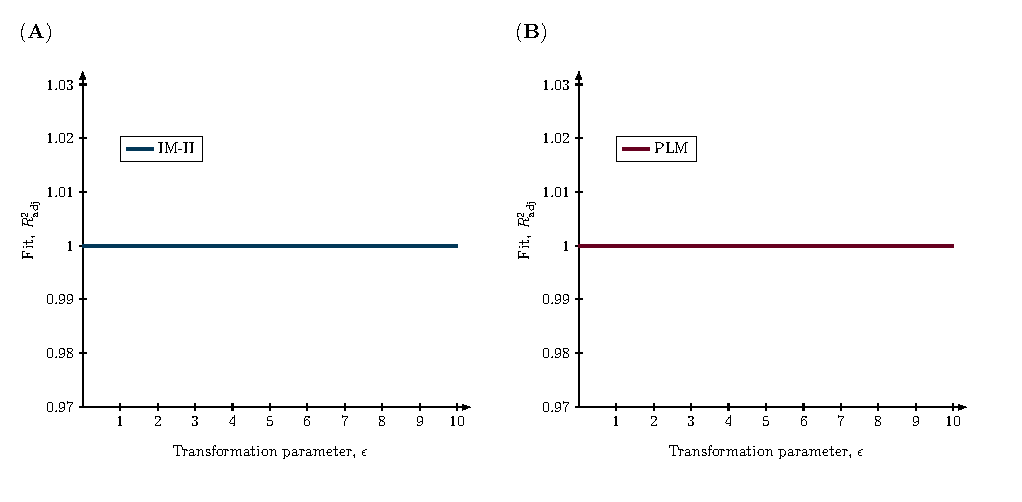
\includegraphics[width=\textwidth]{FigS5}
  \caption[Numerical validation of the symmetries]{\textit{Numerical validation of the symmetries}. The validation of the $t$-directional symmetries of the PLM and the IM-II is done in two steps. Firstly, each curve is transformed with a transformation parameter $\epsilon$. Secondly, the fit of the model to the the transformed data denoted by $R^2_{\mathrm{adj}}(\epsilon)$ is reported. In both cases, it is clear that $R^2_{\mathrm{adj}}\approx 1$ for all tested value of the transformation parameter $\epsilon$. The two tested symmetries are (\textbf{A}) $\Gamma_2$ for the IM-II and (\textbf{B}) $\Gamma_{1,1}$ for the PLM. The family of curves which these symmetries act on are defined by the parameters (\textbf{A}) $(\tau,\alpha)=(67.1564,0.044)$ in the case of the IM-II and (\textbf{B}) $\gamma=5.5600$ in the case of the PLM. The fit have been tested for 100 transformation parameters in the range $\epsilon\in [0,10]$. } 
  \label{fig:numerical_validation}
  \end{figure}



  The numerical validation of the $t$-directional symmetries of the PLM and the IM-II show that they are indeed symmetries. The fit of the models to the transformed solutions is $R^{2}_{\mathrm{adj}}(\epsilon)\approx 1$ (Fig \ref{fig:numerical_validation}) in both cases for a range of transformation parameters $\epsilon$. This illustrates that the scaling symmetry $\Gamma_{1,1}$ in the case of the PLM and the symmetry $\Gamma_{2}$ in case of the IM-II maps solution curves to other solution curves which is the defining property of a symmetry. 
